\documentclass[11pt]{article}

\usepackage[T1]{fontenc}
\usepackage{lmodern}
\usepackage[margin=1in]{geometry}
\usepackage{amsmath,amssymb,amsthm}
\usepackage{booktabs}
\usepackage{microtype}
\usepackage[hidelinks]{hyperref}
\usepackage[round]{natbib}
\usepackage{xcolor}
\usepackage{multirow}
\usepackage{tikz}

\bibliographystyle{apalike}

\newcommand{\E}{\mathbb{E}}
\newcommand{\Prob}{\mathbb{P}}
\newcommand{\R}{\mathbb{R}}
\newcommand{\dw}{d_{W,K}}

\title{Wasserstein Causal Forests: Distribution-Valued Outcomes\\ under Covariate-Dependent Treatment Assignment}
\author{Hugo Gobato Souto\\ Dell Technologies\\ \texttt{hugo.souto@dell.com}}
\date{September 2026}

\begin{document}
\maketitle

\begin{abstract}
We propose Wasserstein Causal Forests (WCF) for observational studies in which each outcome is a probability distribution. WCF estimates the conditional law of potential quantile functions using particle boosting with shared treatment-arm partitions and monotone projection. An augmented inverse-propensity calibration step provides doubly robust scores for population and moderator-specific effects on distributional functionals. We introduce reference-distance effects that measure whether treatment moves the outcome distribution closer to a prespecified benchmark, and an optional two-part representation for a structural zero component. In simulations with covariate-dependent assignment and 1,000 training observations, reference-distance conditional-effect errors range from 0.030 to 0.046 for WCF, compared with 0.133 to 0.248 for Causal-DRF across three location and shape-effect regimes. Additional symmetric and nonlinear designs reveal variation in the ranking across estimands. The results support WCF as a conditional-law learner with functional calibration under observed confounding, while delimiting its performance under finite particle budgets and limited overlap.
\end{abstract}

\section{Introduction}\label{sec:intro}

Average treatment effects reduce an intervention to a difference in means, although many policy and scientific questions concern changes in dispersion, tail behavior, participation, or other features of an outcome law. Conditional distributional treatment effects formalize these questions by comparing potential-outcome distributions or functionals of those distributions. Recent work studies conditional distributional effects through kernel conditional mean embeddings and U-statistic regression \citep{CATEGeneralization}, counterfactual mean embeddings \citep{Counterfactualmeanembeddings}, robust regression of distributional effect pseudo-outcomes \citep{GRFDistributionalCausalEffects}, kernel treatment-effect tests \citep{martineztaboada2023efficient}, and distributional random forests \citep{DRF-paper,naf2026causaldrf}. These approaches establish a methodological basis for asking causal questions about outcomes whose distributional structure is scientifically relevant.

We study the related problem in which the observed outcome for each unit is itself a distribution-valued object, represented here by a quantile function on a common grid. The Wasserstein geometry of quantile functions gives a natural metric for comparing such objects, while particle representations allow the conditional law of the quantile function to retain heterogeneity across units. The proposed Wasserstein Causal Forest combines this representation with a shared treatment-arm partition and a calibration step for scalar functionals of the law. The shared partition is intended for settings in which the treatment probability varies across covariates that also predict the potential-outcome law. The propensity score is the assignment probability $e(x)=\Pr(A=1\mid X=x)$ \citep{rosenbaum1983propensity}; covariate-dependent assignment becomes a source of confounding when those same covariates are prognostic and are not adequately adjusted for.

We study transformed average and conditional average treatment effects (TATE and TCATE), including two reference-distance estimands. Let $Q^a$ denote the potential-outcome quantile vector for a unit, let $q_\star$ be a prespecified reference quantile vector, and let $d_W$ denote the grid Wasserstein distance. The reference-adjusted marginal effect is
\[
\mathrm{TATE}_{\mathrm{ref}}
=\E\left[d_W(Q^1,q_\star)-d_W(Q^0,q_\star)\right],
\]
so a negative value indicates that treatment moves the unit-level outcome distribution closer to the reference on average. Its conditional analogue replaces the outer expectation by conditioning on $X=x$ or on a moderator stratum, giving a reference-adjusted TCATE. These contrasts express improvement or deterioration relative to a substantively chosen benchmark.

The contribution is threefold. First, WCF provides a concrete Wasserstein and quantile representation for conditional laws of distribution-valued outcomes. Second, it combines a common treatment-arm partition with a standard augmented inverse-propensity score for calibration of arbitrary reported functionals. The calibration is doubly robust in the usual nuisance-model sense for each functional when either the propensity nuisance or the corresponding conditional functional regression is consistently estimated \citep{bang2005doubly,chernozhukov2018double}. Third, the paper introduces the reference-adjusted TATE and TCATE contrasts and gives an optional two-part assembly for laws with an exact-zero component. The extension applies when some units have an entirely degenerate outcome distribution, as distinguished from individual zeros within a nondegenerate distribution.

We evaluate WCF in simulation studies designed to vary the treatment effect on location and distributional shape, the degree of overlap, the relationship between treatment assignment and prognostic covariates, and the presence of a point mass. The simulation design is stated directly in terms of the data-generating process. Income and wage distributions provide one interpretation of the quantile-valued outcome, but the same mathematical object can arise for regional expenditure distributions, health-care costs, benefit amounts, or any setting in which a unit is summarized by a distribution and an intervention acts on that distribution. For example, a regional income distribution may respond to a policy through changes in location, dispersion, or participation.

\section{The Wasserstein Causal Forest Model}\label{sec:model}

\subsection{Observed data, representation, and estimands}\label{sec:setup}

We observe independent units $O_i=(X_i,A_i,Q_i)$, where $X_i\in
\mathbb{R}^{d}$ is a vector of pre-treatment covariates, $A_i\in\{0,1\}$ is
the treatment indicator, and $Y_i$ is a probability distribution on $\mathbb{R}$ with finite second moment. We observe its quantile representation $Q_i=q_K(Y_i)$ on a
fixed grid $0<u_1<\cdots<u_K<1$. Writing $Q_Y$ for the quantile function of $Y$, the grid representation is
$q_K(Y)=(Q_Y(u_1),\ldots,Q_Y(u_K))\in\mathcal{Q}_K$, where
$\mathcal{Q}_K=\{q\in\mathbb{R}^K:q_1\leq\cdots\leq q_K\}$. Let
$w_k>0$ and $\sum_k w_k=1$. We use the weighted finite-grid geometry
\[
 d_{W,K}(q,q')=\left\{\sum_{k=1}^{K}w_k(q_k-q'_k)^2\right\}^{1/2}.
\]
This is a quadrature approximation to one-dimensional $W_2$
\citep{peyre2019optimaltransport}; all
estimands below refer to this finite-grid representation. It is also exactly the Wasserstein distance between the discrete distributions $\sum_k w_k\delta_{q_k}$ and $\sum_k w_k\delta_{q_k'}$. Sampling error in estimating each unit's quantile curve is outside the simulation design.

Write $Y^a$ for the potential outcome under treatment level $a$ and
$e(x)=\Pr(A=1\mid X=x)$ for the propensity score \citep{rosenbaum1983propensity}. The identification
conditions are consistency, conditional exchangeability
$Y^a\perp A\mid X$, and positivity $0<e(X)<1$ almost surely. Under these
conditions the arm-specific conditional law
\[
 P_a^K(x)=\operatorname{Law}\{q_K(Y^a)\mid X=x\}
 =\operatorname{Law}\{q_K(Y)\mid A=a,X=x\}
\]
is identified. The method estimates this law directly and subsequently
integrates measurable grid functionals against it.

For a measurable scalar functional $h:\mathcal{Q}_K\to\mathbb{R}$ satisfying $\mathbb{E}|h(q_K(Y^a))|<\infty$ for both arms, define
\[
 \mu_{a,h}(x)=\mathbb{E}\{h(q_K(Y^a))\mid X=x\},\qquad
 \theta_h=\mathbb{E}\{\mu_{1,h}(X)-\mu_{0,h}(X)\},
\]
and, for a pre-treatment moderator $V=g(X)$,
\[
 \tau_h(v)=\mathbb{E}\{\mu_{1,h}(X)-\mu_{0,h}(X)\mid V=v\}.
\]
We call $\theta_h$ the transformed average treatment effect (TATE) and
$\tau_h(v)$ the transformed conditional average treatment effect (TCATE).
For discrete moderators, only strata with positive population probability are considered.
The four functionals used in the experiments are
\begin{align*}
 h_{\mathrm{mean}}(q)&=\bar q=\sum_k w_kq_k,&
 h_{\mathrm{sd}}(q)&=\left\{\sum_k w_k(q_k-\bar q)^2\right\}^{1/2},\\
 h_{\mathrm{skew}}(q)&=\frac{\sum_k w_k(q_k-\bar q)^3}{h_{\mathrm{sd}}(q)^3},&
 h_{\mathrm{tail}}(q)&=\frac{\sum_{k>\lfloor K/2\rfloor}w_kq_k}{\sum_{k>\lfloor K/2\rfloor}w_k}.
\end{align*}
Skewness is assigned the value zero for a constant quantile vector; the upper-half functional includes the middle grid point when $K$ is odd.
The identity
functional $h(q)=q$ gives the mean-quantile contrast
\[
 \tau_q(x)=\mathbb{E}\{q_K(Y^1)-q_K(Y^0)\mid X=x\},
\]
which is a vector-valued barycenter contrast and is distinct from nonlinear
outcome-level functionals of the barycenter.

The reference-distribution estimands use the scalar functional
\[
 h_{\mathrm{ref}}(q)=d_{W,K}(q,q_\star),
\]
where $q_\star$ is a fixed benchmark quantile vector. Thus
\[
 \theta_{\mathrm{ref}}=\mathbb{E}\{h_{\mathrm{ref}}(q_K(Y^1))
 -h_{\mathrm{ref}}(q_K(Y^0))\},\qquad
 \tau_{\mathrm{ref}}(v)=\mathbb{E}\{h_{\mathrm{ref}}(q_K(Y^1))
 -h_{\mathrm{ref}}(q_K(Y^0))\mid V=v\}.
\]
These are the reference-distance TATE and TCATE, respectively. A negative
value means that treatment moves the outcome law closer to the benchmark on
average within the relevant population. They are differences of expected
distances, not the distance between an expected quantile vector and the
benchmark.

Covariate-dependent treatment assignment can induce differences in the distribution of prognostic covariates between arms. Assignment may depend on the untreated mean, on covariates governing dispersion, or on other features of the potential-outcome laws. These are selection-on-observables mechanisms covered by conditional exchangeability. Dependence on unobserved potential-outcome information beyond $X$ requires additional identifying assumptions.

\subsection{Particle-law estimation}\label{sec:boosting}

For each arm, the fitted conditional law is an empirical particle law
\[
 \widehat P_{a,M}^K(x)=\frac{1}{M}\sum_{m=1}^{M}\delta_{p_{am}(x)},
 \qquad p_{am}(x)\in\mathcal{Q}_K.
\]
The particles are fitted by gradient boosting \citep{friedman2001greedy} on the collision-smoothed
energy score
\[
 S_\varepsilon(P,q)=\frac{1}{M}\sum_{m=1}^{M}d_{\varepsilon}(p_m,q)
 -\frac{1}{2M^2}\sum_{m,l=1}^{M}d_{\varepsilon}(p_m,p_l),
 \qquad
 d_{\varepsilon}(a,b)=\{d_{W,K}(a,b)^2+\varepsilon^2\}^{1/2}-\varepsilon.
\]
The unsmoothed energy score is strictly proper for probability laws on the weighted Euclidean space under a finite first-moment condition \citep{gneiting2007proper}. Finite particle count, smoothing, and the tree function class restrict the implemented optimization. The first term attracts the particle cloud to the observed quantile vector and
the second term preserves dispersion. At iteration $t$, only the observed arm contributes a gradient for unit $i$. The tree response for particle $m$ and coordinate $k$ is the preconditioned descent direction
\[
 G_{imk}=-\frac{M}{w_k}\frac{\partial S_\varepsilon(P,Q_i)}{\partial p_{mk}}
 \bigg|_{P=\widehat P_{A_i,M}^{K,(t)}(X_i)}.
\]
The shared tree maps $X_i$ to an arm-specific vector in $\mathbb{R}^{M K}$. For each arm, its update $g_a^{(t)}(x)$ produces
\[
 p_{am}^{(t+1)}(x)=\Pi_{\mathcal Q_K}^{w}\{p_{am}^{(t)}(x)+\eta_t g_{am}^{(t)}(x)\},
\]
where $\Pi_{\mathcal Q_K}^{w}$ is weighted isotonic projection, computed by the pool-adjacent-violators algorithm \citep{barlow1972isotonic}. A backtracking search halves $\eta_t$ until the observed-arm training score does not increase, up to numerical tolerance; fitting stops if no acceptable step is found. Prediction applies the fitted updates and projection in the same order.
The particle representation
estimates an arm-specific conditional law. It does not identify a coupling of
$Y^0$ and $Y^1$, and differences between matched particles from the two arms
are not individual treatment effects.

The final learner uses a shared covariate partition. Candidate splits are
scored with the pooled multi-output squared-error criterion and are retained
only when each child contains the required number of observations from each
arm. For the contrast-regularized update used in WCF, let $g_a$ be the
mean descent target in a leaf for arm $a$, let $n_a$ be its arm count, let
$\bar g=(n_0g_0+n_1g_1)/(n_0+n_1)$, and let $\delta=g_1-g_0$. With
$n_{\mathrm{eff}}=n_0n_1/(n_0+n_1)$ and
$c_\lambda=n_{\mathrm{eff}}/(n_{\mathrm{eff}}+\lambda)$, the leaf updates are
\[
 \widehat g_0=\bar g-\frac{n_1}{n_0+n_1}c_\lambda\delta,
 \qquad
 \widehat g_1=\bar g+\frac{n_0}{n_0+n_1}c_\lambda\delta.
\]
This shrinks the arm gap while preserving the count-weighted pooled gradient.
The strength $\lambda$ is selected from a fixed candidate set by held-out
energy risk computed only on each validation unit's observed arm. The method
initializes both arms with the same $M$ quantile vectors, selected at equally spaced ranks from the lexicographically ordered pooled training vectors. The common initialization starts the arm contrast at zero.

Figure~\ref{fig:pipeline} summarizes the two outputs of WCF.
\begin{figure}[t]
\centering
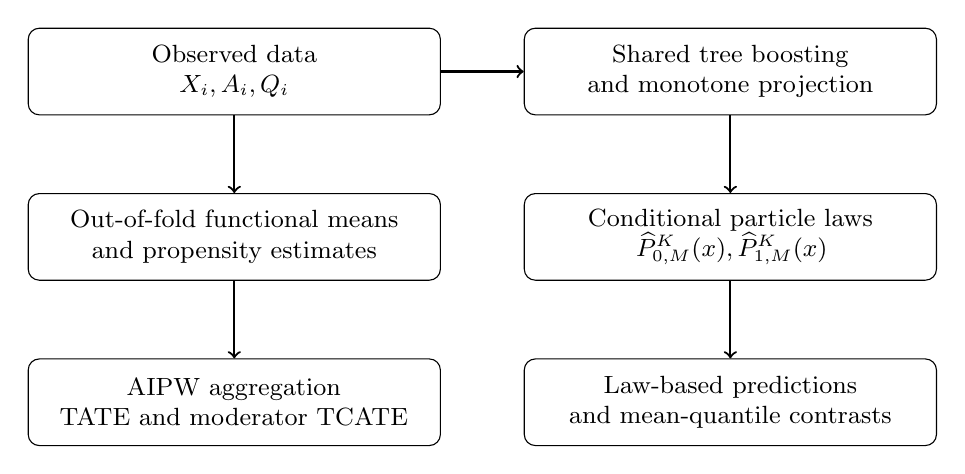
\begin{tikzpicture}[every node/.style={font=\small},box/.style={draw,rounded corners,align=center,text width=5cm,minimum height=1.1cm}]
\node[box] (data) at (0,0) {Observed data\\$X_i,A_i,Q_i$};
\node[box] (fit) at (6.3,0) {Shared tree boosting\\and monotone projection};
\node[box] (laws) at (6.3,-2.1) {Conditional particle laws\\$\widehat P_{0,M}^K(x),\widehat P_{1,M}^K(x)$};
\node[box] (nuisance) at (0,-2.1) {Out-of-fold functional means\\and propensity estimates};
\node[box] (effects) at (0,-4.2) {AIPW aggregation\\TATE and moderator TCATE};
\node[box] (lawoutputs) at (6.3,-4.2) {Law-based predictions\\and mean-quantile contrasts};
\draw[->,thick] (data) -- (fit);
\draw[->,thick] (data) -- (nuisance);
\draw[->,thick] (fit) -- (laws);
\draw[->,thick] (nuisance) -- (effects);
\draw[->,thick] (laws) -- (lawoutputs);
\end{tikzpicture}
\caption{WCF produces conditional laws and calibrated functional contrasts. The calibration uses out-of-fold particle fits and propensity estimates. It adjusts the functional contrasts without changing the final particle laws.}
\label{fig:pipeline}
\end{figure}


\subsection{Doubly robust calibration of scalar functionals}\label{sec:dr}

The particle law and the functional calibration layer target different
objects. For a declared functional $h$, let $\widehat m_{a,h}^{(-k)}(X_i)$
be the out-of-fold mean of $h$ over the fitted arm-$a$ particles, and let
$\widetilde e_i$ be a cross-fitted propensity estimate bounded away from zero and one. With $H_i=h(q_K(Y_i))$, define
\[
 \widehat\phi_i(h)=\widehat m_{1,h}^{(-k)}(X_i)
 -\widehat m_{0,h}^{(-k)}(X_i)
 +\frac{A_i}{\widetilde e_i}
   \{H_i-\widehat m_{1,h}^{(-k)}(X_i)\}
 -\frac{1-A_i}{1-\widetilde e_i}
   \{H_i-\widehat m_{0,h}^{(-k)}(X_i)\}.
\]
The marginal estimator is the sample mean of $\widehat\phi_i(h)$ and the
moderator-specific estimator is its sample mean within the observed bin
$V=v$. In the implementation, WCF applies this layer to the four grid
functionals and $h_{\mathrm{ref}}$. It replaces their reported contrast
columns, while the particle laws and all law-level scores remain those of the
particle booster.

The augmented score follows standard doubly robust estimation and cross-fitting \citep{bang2005doubly,chernozhukov2018double}. For fixed nuisance limits $m_a^\dagger$ and $e^\dagger$, the conditional bias
of the corresponding population score is
\[
 (e^\dagger-e(X))\left[
 \frac{m_1^\dagger(X)-\mu_{1,h}(X)}{e^\dagger}
 +\frac{m_0^\dagger(X)-\mu_{0,h}(X)}{1-e^\dagger}
 \right].
\]
Consequently, the score has the standard doubly robust property at the level
of the scalar functional: the bias vanishes when the propensity is correct or
when both arm-specific conditional means are correct, subject to positivity,
integrability, and the usual conditions controlling nuisance estimation and
cross-fitting. The robustness property applies to the calibrated averages; the conditional particle laws and pointwise mean-quantile contrasts remain outcome-model estimates. With fixed $M$, the functional means induced by a particle fit need not consistently approximate every chosen functional. The score identity therefore provides a robustness route, not a guarantee that the fixed-budget learner satisfies either nuisance-correctness condition.

The propensity nuisance may be estimated with any binary probability model whose predictions satisfy the required overlap and convergence conditions. Logistic regression is a working choice for the experiments. Flexible classifiers can accommodate nonlinear assignment, with tuning confined to the appropriate training samples. Fixed propensity clipping can introduce bias when it excludes part of the true propensity range. Valid asymptotic inference additionally requires moment, nuisance-rate, and sample-splitting conditions; score unbiasedness alone is insufficient to establish efficiency.

\subsection{Optional two-part law for a degenerate component}\label{sec:zipt}

Some distribution-valued outcomes have a structural component in which the
entire unit-level outcome law is degenerate at a point. For example, a facility's expenditure distribution may be identically zero during an inactive period and nondegenerate during an active period. Participation and intensity are commonly separated in economic two-part models, including medical expenditure and count models \citep{duan1983medical,mullahy1986modified}. Here the mixture operates on distribution-valued observations: an atom at the all-zero quantile vector differs from a positive fraction of individuals with zero expenditure inside every unit's distribution. For such data, the optional two-part extension
estimates
\[
 \pi_a(x)=\Pr\{q_K(Y^a)\neq\mathbf{0}\mid X=x\}
\]
with an arm-specific binary classifier, fits the particle booster on the
nondegenerate rows, and assembles
\[
 \widehat P_a^{\mathrm{2p}}(x)=
 \{1-\widehat\pi_a(x)\}\delta_{\mathbf{0}}
 +\widehat\pi_a(x)\widehat P_{a,M}^{+,K}(x).
\]
The extension gives the degenerate component its own estimable probability
and lets every downstream law functional integrate over both parts. The plain
particle booster can place mass exactly at zero, but it has no
separate component-probability parameter and its particle masses are tied to
$1/M$; the two-part assembly makes that structural mass explicit. The extension can be enabled when the data contain this structural component. Its evaluation below concerns the assembled law and component probabilities; it does not assess an additional AIPW calibration of the mixture.
